%====================================================
%
% Author: Dipl.-Inf. Xavier NOUMBISSI NOUNDOU, Ph.D.-Candidate
% Email:  xnoundou7@gmail.com
%
%====================================================
\documentclass[12pt, a4paper]{article}
\NeedsTeXFormat{LaTeX2e}

%---------------------------- PACKAGE INCLUSION -------------------------------
% This group renders characters clearer and more precise

\RequirePackage[bitstream-charter,cal,expert]{mathdesign}
\RequirePackage{latexsym}

\usepackage{geometry}
\geometry{a4paper,
		  %showframe=true,
		  %margin=2.75em,
		  %a4paper,
		  %total={170mm,257mm},
		  top=3.5em,
		  left=3em,
		  right=3em,
		  bottom=3.39em
		  }

\usepackage[default]{cantarell}
\usepackage{graphicx}
\usepackage{xspace}
\usepackage[parfill]{parskip} % Activate to begin paragraphs with an empty line rather than an indent
\usepackage{paralist} % very flexible & customisable lists (eg. enumerate/itemize, etc.)
\usepackage{listings} % for lstset definitions
\usepackage{url}
\usepackage{subfig} % make it possible to include more than one captioned figure/table in a single float
\usepackage{epsfig}
\usepackage{booktabs}
%\usepackage{enumitem} %funny itemize icons
\usepackage{verbatim}
\usepackage{tcolorbox}

\usepackage{pagecolor}

\usepackage{amsmath}
\newcommand{\mathbold}[1]{\text{\textbf{#1}}}

\usepackage{xcolor}
\definecolor{yerenColorOrange}{RGB}{242, 161, 0}   
\definecolor{yerenColorBlue}{RGB}{77 , 93 , 254}
\definecolor{yerenColorRed}{RGB}{254, 48 , 48}
\definecolor{yerenColorGray}{RGB}{197, 197, 197}
\definecolor{yerenColorDarkgray}{RGB}{60, 60 , 60}
\definecolor{yerenColorIndigo}{RGB}{83, 0, 125}
\definecolor{yerenColorGreen}{RGB}{2, 160, 70}
\definecolor{forestgreen}{RGB}{2,160,70}    
\definecolor{mediumblue}{RGB}{7,43,205}    
\definecolor{firebrickred}{RGB}{178,34,34}
\definecolor{listingray}{gray}{0.9}
\definecolor{lbcolor}{rgb}{0.9,0.9,0.9}
\definecolor{darkgreen}{rgb}{0,0.35,0}
\definecolor{medgreen}{rgb}{0,0.5,0}
\definecolor{lightgreen}{rgb}{0.5,0.7,0.5}
\definecolor{pmcolour}{rgb}{0.5,0.7,0.5}
\definecolor{medgrey}{rgb}{0.6,0.6,0.6}
\definecolor{purplish}{rgb}{0.4,0,0.6}
\definecolor{brightred}{rgb}{1,0.2,0.2}

\newcommand{\diplinfn}{Dipl.--Inf.\xspace}

\newcommand{\yerenlabs}{\textsc{YEROTH~R\&D}\xspace}

\newcommand{\yerenpos}{\textcolor{yerenColorBlue}{\sc YEROTH--ERP--$3.0$}\xspace}

\newcommand{\myfullacademicname}{Xavier NOUMBISSI NOUNDOU, Ph.D. (ABD)\xspace}

\usepackage{hyperref}
\hypersetup{
    colorlinks,
	pagebackref,
    citecolor=medgreen,
    linkcolor=purplish,
    breaklinks,
    pdftex,
    bookmarks,
    plainpages=false,
	pdftitle={\yerenpos software--system product sheet authored by: ''\myfullacademicname''},
    pdfauthor={Xavier NOUMBISSI NOUNDOU}
}

%--------------------------------------------------------------------------------

%---------------------------- COMMANDS DEFINITION -------------------------------
\newcommand{\diplinf}{\emph{Dipl.-Inf.}\xspace}
\newcommand{\mycheckmark}[1]{\textcolor{#1}{$\checkmark$}\xspace}

\newcommand{\myenumitem}[1]{\emph{#1}\xspace}
\newcommand{\yerenalert}{\emph{yeren-alert}\xspace}

\newcommand{\pos}{ERP~software--system\xspace}

\newcommand{\mysql}{MySQL\xspace}
\newcommand{\mysqlcolored}{\textcolor{yerenColorBlue}{My}\textcolor{yerenColorOrange}{SQL}\xspace}

\newcommand{\admin}{<< Administrator >>\xspace}
\newcommand{\manager}{<< Manager >>\xspace}
\newcommand{\seller}{<< Seller >>\xspace}
\newcommand{\inventorystockmanager}{<< InventoryStockManager >>\xspace}
\newcommand{\storekeeper}{<< StoreKeeper >>\xspace}
\newcommand{\cashier}{<< Cashier >>\xspace}

\newcommand{\adminb}{\textbf{<< Administrator >>}\xspace}
\newcommand{\managerb}{\textbf{<< Manager >>}\xspace}
\newcommand{\inventorystockmanagerb}{\textbf{<< InventoryStockManager >>}\xspace}
\newcommand{\storekeeperb}{\textbf{<< StoreKeeper >>}\xspace}
\newcommand{\cashierb}{\textbf{<< Cashier >>}\xspace}

\newcommand{\featuresummary}[2]{\textbf{\textcolor{#1}{\textsc{#2}}}}

%--------------------------------------------------------------------------------

\usepackage[T1]{fontenc}
\newcommand{\changefont}[3]{
\fontfamily{#1} \fontseries{#2} \fontshape{#3} \selectfont}
\changefont{cmss}{m}{n}

\renewcommand\labelenumi{\theenumi)}

\pagenumbering{gobble}

\usepackage{fancyhdr}
\pagestyle{fancy}
\renewcommand{\headrulewidth}{0pt}
\rhead{}
\lhead{}
\cfoot{}

\clubpenalty = 10000
\widowpenalty = 10000
\displaywidowpenalty = 10000

\begin{document}

{\bf \LARGE \yerenpos} {| \sc \scriptsize software--system product sheet }

\vspace{3.75em}

\begin{table}[!htbp]
\begin{tabular}{ll}
\parbox{27em}{

\yerenpos is an \textbf{\pos} with $6$ \textbf{user roles, and types}:
\vspace{0.1em}
\begin{enumerate}
	\item \admin
	\item \manager
	\item \seller
	\item \inventorystockmanager
	\item \cashier
	\item \storekeeper.\\
\end{enumerate}

\yerenpos \textbf{features}:
\vspace{0.1em}
\begin{enumerate}
	\item inventory--stock--management
	\item alerts over stock--quantity, and, time--period	
	\item stock--buying--management
	\item sale--management (stock--checkout, etc.)
	\item customer--relationship--management
	\item business dashboard
	\item user--, and role--administration.\\
\end{enumerate}

\yerenpos \textbf{is}:
\vspace{0.1em}
\begin{enumerate}
	\item lighter, and, faster, in memory--usage
	\item easier, and, intuitiver, in its use
	\item multi--sites (enabled).\\
\end{enumerate}

\vspace{0.5em}

\yerenpos's runtime memory usage test is realized
using software--analysis tool \textbf{valgrind}.\\
}

&

\parbox{15em}{
\begin{center}
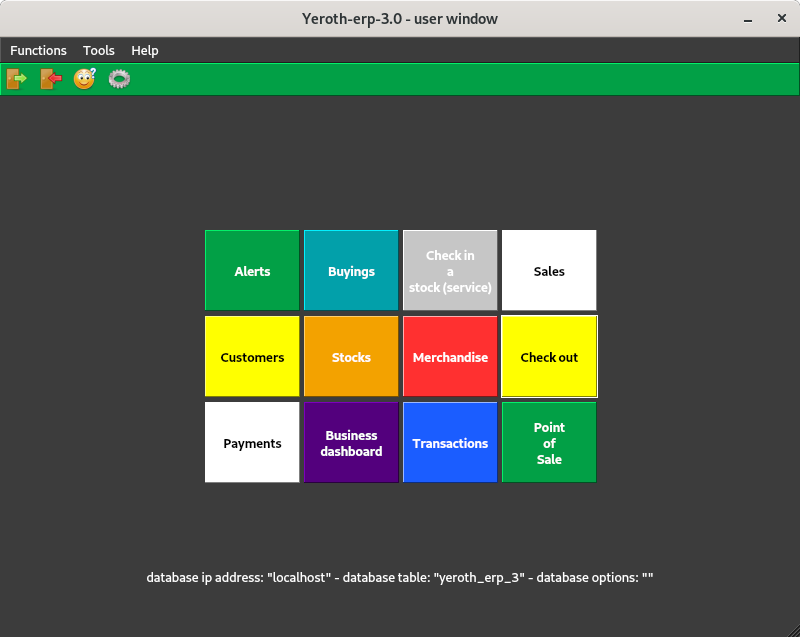
\includegraphics[scale=0.25]{images/yeroth-manager-window.png}
\caption*{Manager's main window}

\vspace{3em}

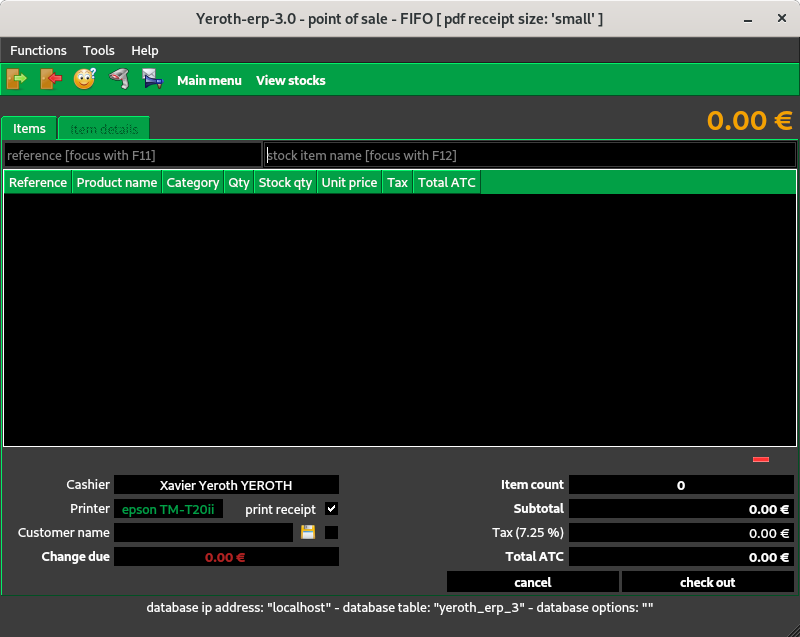
\includegraphics[scale=0.25]{images/yeroth-cashier-window.png}
\caption*{Cashier's main window}

\end{center}
}
\end{tabular}
\end{table}

\vspace{1.25em}

{\large \bf OPERATIONS}

\vspace{0.75em}

\begin{table}[!htbp]
\begin{tabular}{lll}

\begin{tcolorbox}[width=14.3em, boxrule=0.01em, colback=white]
\textbf{Point--of--Sale Hardware}
\vspace{-1em}
\hrule
\vspace{0.75em}
\begin{itemize}[]
	\item[\mycheckmark{yerenColorDarkgray}] Barcode scanner
	\item[\mycheckmark{yerenColorDarkgray}] Thermal printer, etc.\\
\end{itemize}
\begin{center}
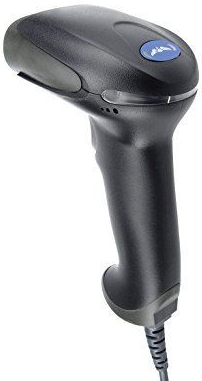
\includegraphics[scale=0.24]{images/xfox-fj-5-usb-plug-and-play-automatic-barcode-scanner.png}
\end{center}
\end{tcolorbox}

&

\begin{tcolorbox}[width=14.3em, boxrule=0.01em, colback=white]
\textbf{Database Management Systems}
\vspace{0.1em}
\hrule
\vspace{0.75em}
\begin{itemize}[]
	\item[\mycheckmark{yerenColorBlue}] \mysqlcolored\\
\end{itemize}
\begin{center}

\includegraphics[scale=0.14]{images/free-reuse-dbms-logo}
\end{center}
\end{tcolorbox}

&

\begin{tcolorbox}[width=14.3em, boxrule=0.01em, colback=white]
\textbf{Operating Systems}
\vspace{0.1em}
\hrule
\vspace{0.75em}
\begin{itemize}[]
	\item[\mycheckmark{yerenColorRed}] Windows~$10$ \& Linux--Debian\\	
\end{itemize}
\begin{center}

\includegraphics[scale=0.47]{images/free-reuse-stretch-logo}
\end{center}
\end{tcolorbox}

\end{tabular}
\end{table}
	
\end{document}

